\documentclass[12pt,a4paper]{article}
%\usepackage{ctex}
\PassOptionsToPackage{unicode}{hyperref}
\PassOptionsToPackage{hyphens}{url}
\usepackage{amsmath,amscd,amsbsy,amssymb,latexsym,url,bm,amsthm}
\usepackage{epsfig,graphicx,subfigure}
\usepackage{enumitem,balance}
\usepackage{wrapfig}
\usepackage{mathrsfs,euscript}
\usepackage[usenames]{xcolor}
\usepackage[colorlinks,linkcolor = blue]{hyperref}
\usepackage[vlined,ruled,commentsnumbered,linesnumbered]{algorithm2e}
\usepackage{listings}
\usepackage[utf8]{inputenc}

\newtheorem{theorem}{Theorem}
\newtheorem{lemma}[theorem]{Lemma}
\newtheorem{proposition}[theorem]{Proposition}
\newtheorem{corollary}[theorem]{Corollary}
\newtheorem{exercise}{Exercise}
\newtheorem*{solution}{Solution}
\newtheorem{definition}{Definition}
\theoremstyle{definition}


%\numberwithin{equation}{section}
%\numberwithin{figure}{section}

\renewcommand{\thefootnote}{\fnsymbol{footnote}}

\newcommand{\postscript}[2]
 {\setlength{\epsfxsize}{#2\hsize}
  \centerline{\epsfbox{#1}}}

\renewcommand{\baselinestretch}{1.0}

\setlength{\oddsidemargin}{-0.365in}
\setlength{\evensidemargin}{-0.365in}
\setlength{\topmargin}{-0.3in}
\setlength{\headheight}{0in}
\setlength{\headsep}{0in}
\setlength{\textheight}{10.1in}
\setlength{\textwidth}{7in}
\makeatletter \renewenvironment{proof}[1][Proof] {\par\pushQED{\qed}\normalfont\topsep6\p@\@plus6\p@\relax\trivlist\item[\hskip\labelsep\bfseries#1\@addpunct{.}]\ignorespaces}{\popQED\endtrivlist\@endpefalse} \makeatother
\makeatletter
\renewenvironment{solution}[1][Solution] {\par\pushQED{\qed}\normalfont\topsep6\p@\@plus6\p@\relax\trivlist\item[\hskip\labelsep\bfseries#1\@addpunct{.}]\ignorespaces}{\popQED\endtrivlist\@endpefalse} \makeatother



\usepackage{color}
\definecolor{codegreen}{rgb}{0,0.6,0}
\definecolor{codegray}{rgb}{0.5,0.5,0.5}
\definecolor{codepurple}{rgb}{0.58,0,0.82}
\definecolor{backcolour}{rgb}{0.95,0.95,0.92}
 
\lstdefinestyle{mystyle}{  
    commentstyle=\color{codegreen},
    keywordstyle=\color{blue},
    numberstyle=\tiny\color{codegray},
    stringstyle=\color{codepurple},
    basicstyle=\footnotesize,
    breakatwhitespace=false,         
    breaklines=true,                 
    captionpos=b,                    
    keepspaces=true,                 
    numbers=left,                    
    numbersep=5pt,                  
    showspaces=false,                
    showstringspaces=false,
    showtabs=false,                  
    tabsize=2,
    frame=shadowbox
}
\lstset{style=mystyle}
\begin{document}

\noindent

%========================================================================
\noindent\framebox[\linewidth]{\shortstack[c]{
\Large{\textbf{Lab03 Sorting and Selection}}\vspace{1mm}\\
VE281 - Data Structures and Algorithms, Xiaofeng Gao, Autumn 2019}}
%VE281 - Data Structures and Algorithms, Xiaofeng Gao, Autumn 2019}}
\begin{center}    
    \footnotesize{\color{blue}Name:Wu Jiayao  \quad Student ID:517370910257 \quad Email: jiayaowu1999@sjtu.edu.cn}
    \end{center}
    
\section{Comparison between five sorting
algorithm}
\par The running time of bubble sort is much more longer than other sorting
algorithm, followed by selection sort, insert sort, merge sort and quick
sort. The difference becomes much more obvious and significant when the
size of the array grows.
\begin{figure}[htbp]
    \centering
    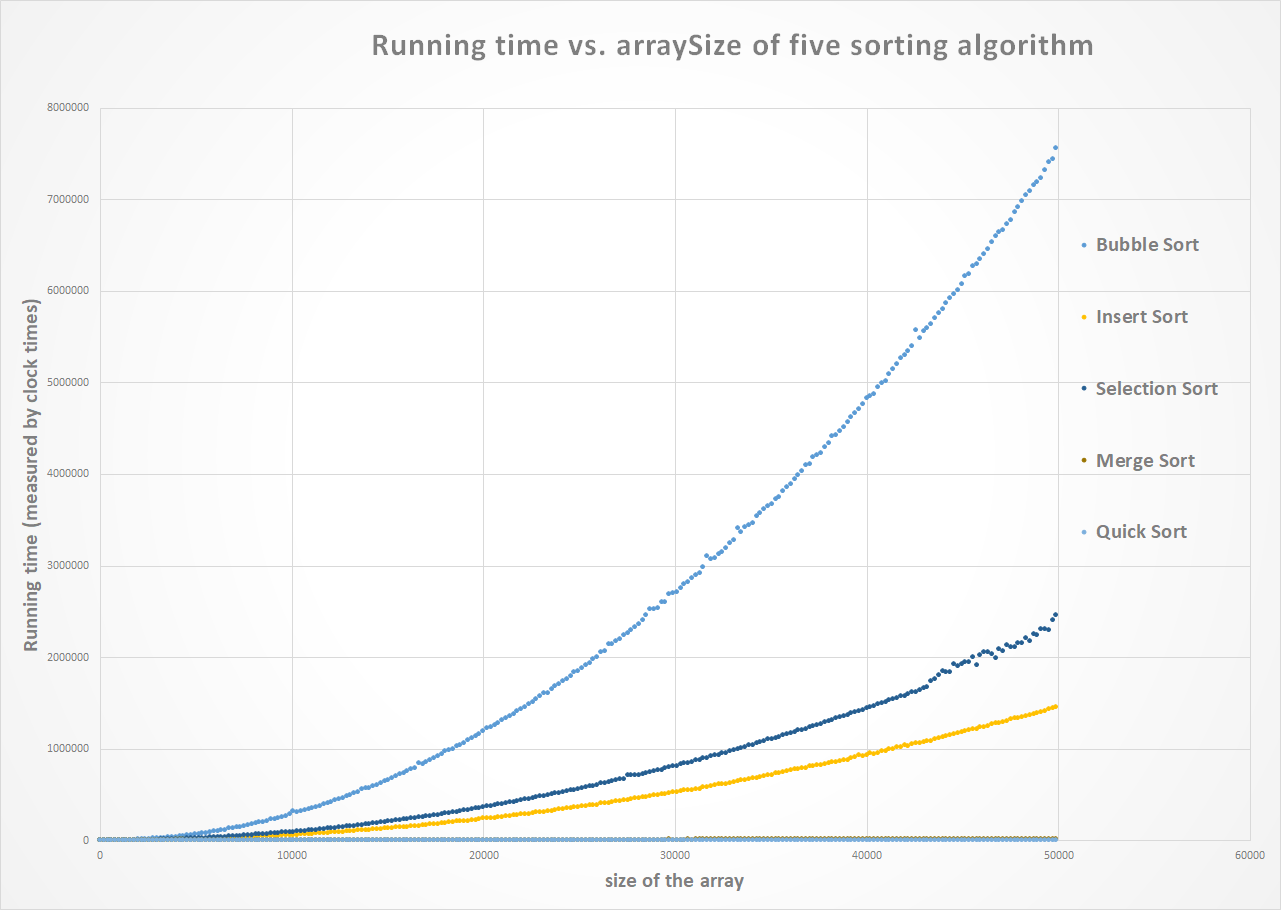
\includegraphics[width=0.95\textwidth]{1.png}
    \caption{Running time vs. size of array for five sorting algorithms}
\end{figure}
\newpage
\par Since the running time of merge sort and quick sort are too closely
plotted to be recognized, here is a plot which only contains running
time of merge sort and quick sort. It can be seen in the figure that quick sort tends to perform better
than merge sort overall.

\begin{figure}[htbp]
    \centering
    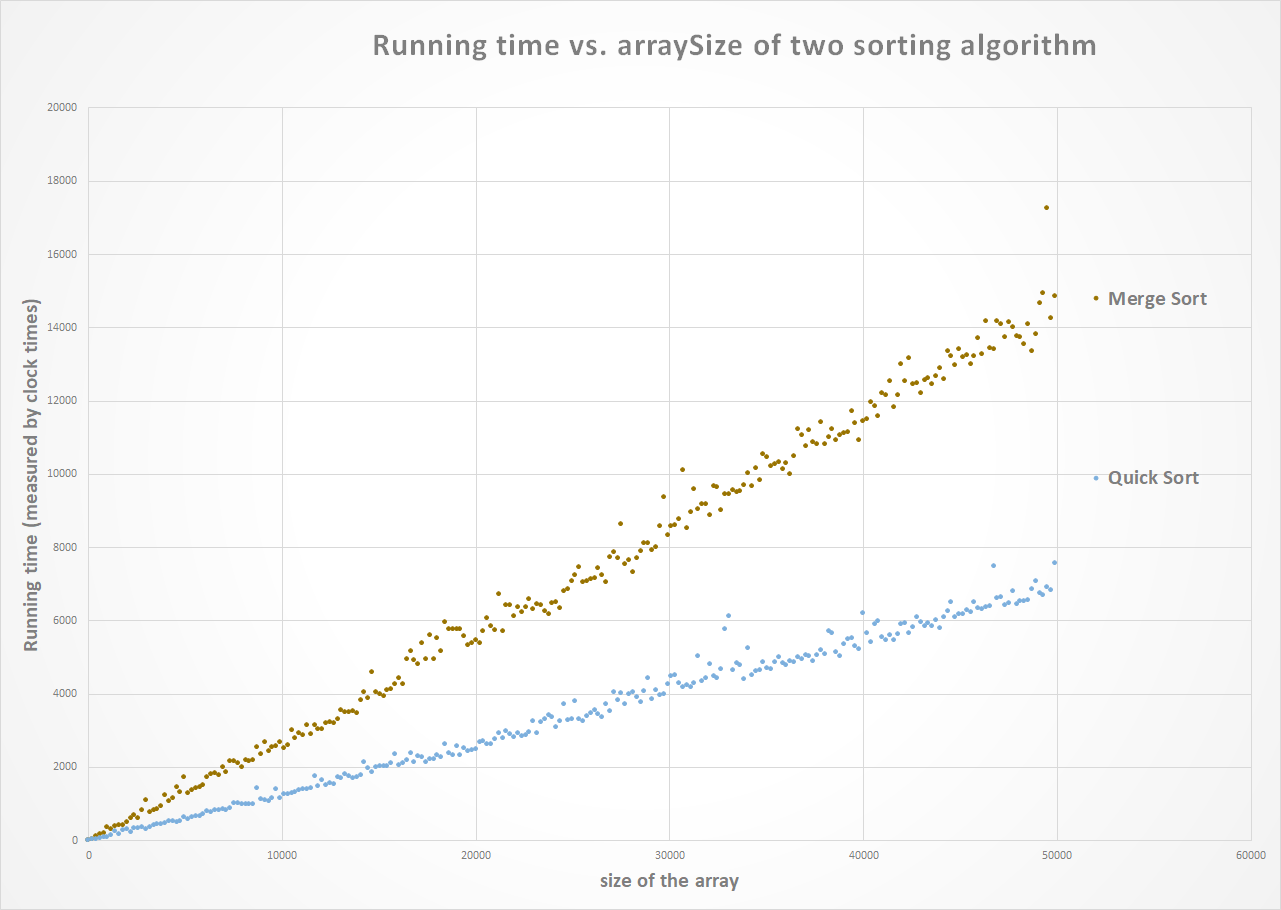
\includegraphics[width=0.95\textwidth]{2.png}
    \caption{Running time vs. size of array for two sorting algorithms}
\end{figure}


\newpage
\section{Comparison between two selection algorithm}
\begin{figure}[htbp]
    \centering
    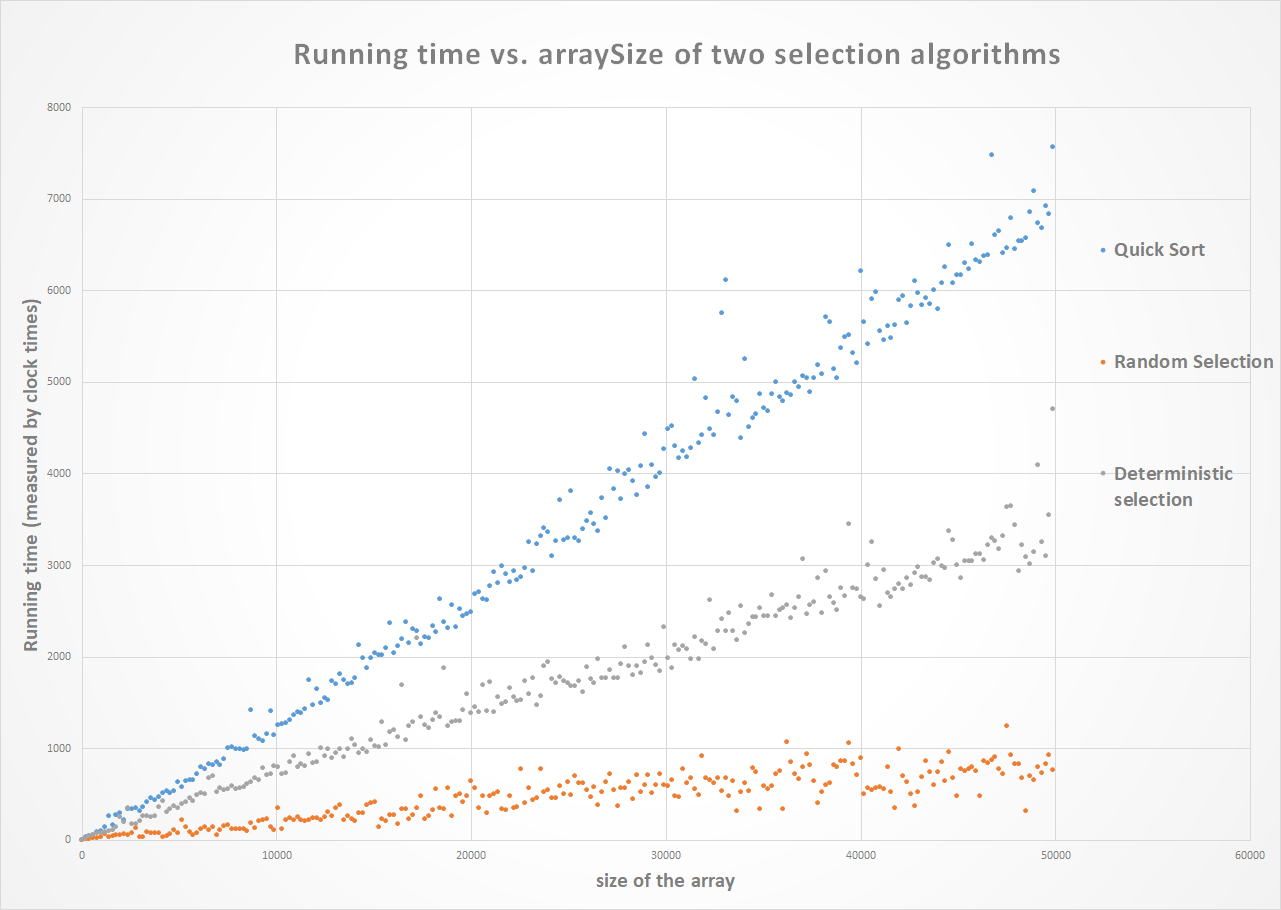
\includegraphics[width=0.95\textwidth]{3.png}
    \caption{Running time vs. size of array for two selection algorithms with quick sort}
\end{figure}

\par In this test, random selection performs better than deterministic
selection in less running time. Both two selection algorithms performs
better than quick sort in less running time. Differences become much
more obvious and significant when the size of the array grows.
\newpage
\section*{Appendix}
\subsection{Source code}
\subsubsection*{sort.h}
\begin{lstlisting}[language=C++]
#ifndef SRC_SORT_H
#define SRC_SORT_H

#include <cstdlib>
#include <iostream>
//#define TIMING
void swap(int, int, int *);
void printArray(int *, int);
void printSearch(int, int);

void bubbleSort(int *, int);

void insertSort(int *, int);

void selectionSort(int *, int);

void mergeSort(int *, int);

void quickSort(int *, int, int);

int rSelect(int *, int, int, int);
int dSelect(int *, int, int, int);

#endif //SRC_SORT_H

\end{lstlisting}
\subsubsection*{bubbleSort.cpp}
\begin{lstlisting}[language=C++]
    #include "sort.h"
    void bubbleSort(int *nums, int length)
    {
        for(int i = 0 ; i<length-1;i++)
        {
            for (int j = 0; j < length-1-i; j++)
            {
                if(nums[j] > nums[j+1])
                {
                    swap(j,j+1,nums);
                }
            }
        }
    }

\end{lstlisting}
\subsubsection*{insertionSort.cpp}
\begin{lstlisting}[language=C++]
    #include "sort.h"
    void insertSort(int* nums, int length){
        for(int i = 1 ; i<length;i++)
        {
            int tmp = nums[i],j = i-1;
            while(j>=0 && tmp < nums[j])
            {
                nums[j+1] = nums[j];
                j--;
            }
            nums[j+1] = tmp;
        }
    
    }   
\end{lstlisting}
\subsubsection*{selectionSort.cpp}
\begin{lstlisting}[language=C++]
    #include "sort.h"

    void selectionSort(int*nums,int length)
    {
        for(int i = 0 ;i < length - 1;i++)
        {
            int min = INT32_MAX;
            int minAt = i;
            for(int j = i ; j< length;j++)
            {
                if(nums[j]<min)
                {
                    min = nums[j];
                    minAt = j;
                }
            }
            swap(i,minAt,nums);
        }
    }
\end{lstlisting}
\subsubsection*{mergeSort.cpp}
\begin{lstlisting}[language=C++]
    #include "sort.h"
    static void merge(int *nums, int *l, int lSize, int *r, int rSize)
    {
        int i = 0, j = 0, itr = 0;
        while (i < lSize && j < rSize)
        {
            if (l[i] < r[j])
            {
                nums[itr++] = l[i++];
            }
            else
            {
                nums[itr++] = r[j++];
            }
        }
        while (i < lSize)
        {
            nums[itr++] = l[i++];
        }
        while (j < rSize)
        {
            nums[itr++] = r[j++];
        }
    }
    void mergeSort(int *nums, int length)
    {
        if (length < 2)
        {
            return;
        }
        int mid = length / 2;
        int *l = new int[mid];
        int *r = new int[length - mid];
        for (int i = 0; i < mid; i++)
        {
            l[i] = nums[i];
        }
        for (int i = mid; i < length; i++)
        {
            r[i - mid] = nums[i];
        }
        mergeSort(l, mid);
        mergeSort(r, length - mid);
        merge(nums, l, mid, r, length - mid);
        delete[] l;
        delete[] r;
    }
\end{lstlisting}
\subsubsection*{quickSort.cpp}
\begin{lstlisting}[language=C++]
    #include "sort.h"
    using namespace std;
    void quickSort(int* nums,int left,int right)
    {
        if(left >= right)
        {
           return ;
        }
        int pivotIndex = rand() % (right - left + 1) + left;
        swap(left,pivotIndex,nums);
        int pivotat = left;
        int i = left + 1, j = i;
        for (; j <= right; j++)
        {
            if (nums[j] < nums[pivotat])
            {
                swap(i,j,nums);
                i++;
            }
        }
        swap(i-1,pivotat,nums);
        quickSort(nums,left, i - 2);
        quickSort(nums,i, right);
    }
\end{lstlisting}
\subsubsection*{selection.cpp}
\begin{lstlisting}[language=C++]
    #include "sort.h"

    int rSelect(int *nums, int left, int right, int k)
    {
        if (left == right)
        {
            return nums[left];
        }
        int index = rand() % (right - left + 1) + left;
        swap(index, left, nums);
        int pivot = nums[left];
        int i = left + 1, j = i;
        for (; i <= right; i++)
        {
            if (nums[i] < pivot)
            {
                swap(j, i, nums);
                j++;
            }
        }
        swap(j - 1, left, nums);
        int relative = (j - 1) - left;
        if (relative == k)
        {
            return nums[j - 1];
        }
        else if (relative > k)
        {
            return rSelect(nums, left, j - 2, k);
        }
        else
        {
            return rSelect(nums, j, right, k - relative - 1);
        }
    }
    
    static int choosePivot(int *nums, int left, int right)
    {
        if (left == right)
        {
            return nums[left];
        }
        int length = right - left + 1;
        int divLength = length % 5 == 0 ? length / 5 : length / 5 + 1;
        int *res = new int[divLength];
        int itr = 0;
        for (int i = 0; i < length; i = i + 5)
        {
            int tmpRight = (i + 4 >= length) ? length - 1 : i + 4;
            int tmpLength = tmpRight - i + 1;
            int *div = new int[tmpLength];
            for (int j = i; j <= tmpRight; j++)
            {
                div[j - i] = nums[j];
            }
            quickSort(div, 0, tmpLength - 1);
            if (tmpLength % 2 == 1)
            {
                res[itr++] = div[tmpLength / 2];
            }
            else
            {
                res[itr++] = (div[tmpLength / 2] + div[tmpLength / 2 - 1]) / 2;
            }
            delete[] div;
        }
        int x = choosePivot(res, 0, divLength - 1);
        delete[] res;
        return x;
    }
    
    int dSelect(int *nums, int left, int right, int k)
    {
        if (left == right)
        {
            return nums[left];
        }
        int pivot = choosePivot(nums, left, right);
        int pivotat = 0;
        for (int i = left; i < right; i++)
        {
            if (nums[i] == pivot)
            {
                pivotat = i;
            }
        }
        swap(pivotat, left, nums);
        //int pivot = nums[left];
        int i = left + 1, j = i;
        for (; i <= right; i++)
        {
            if (nums[i] < pivot)
            {
                swap(j, i, nums);
                j++;
            }
        }
        swap(j - 1, left, nums);
        if (j - 1 == k)
        {
            return nums[k];
        }
        else if (j - 1 > k)
        {
            return rSelect(nums, left, j - 2, k);
        }
        else
        {
            return rSelect(nums, j, right, k - j + 1);
        }
    }
\end{lstlisting}
\subsubsection*{basic\_operations.cpp}
\begin{lstlisting}[language=C++]
    #include "sort.h"
    using namespace std;
    void swap(int a,int b,int* nums)
    {
        int tmp = nums[a];
        nums[a] = nums[b];
        nums[b] = tmp;
    }
    void printArray(int* nums,int length)
    {
        for(int i = 0 ; i < length;i++)
        {
            cout << nums[i] << endl;
        }
    }
    
    void printSearch(int key,int value)
    {
        cout << "The order-" << key <<" item is " << value << endl;
    }
\end{lstlisting}
\subsubsection*{main.cpp}
\begin{lstlisting}[language=C++]
    #include "sort.h"
    #ifdef TIMING
    #include <time.h>
    #endif
    using namespace std;
    int main()
    {
        int mode = 0;
        cin >> mode;
        int length = 0;
        cin >> length;
        int select = 0;
    
        int *nums = new int[length];
        if (mode == 5 || mode == 6)
        {
            cin >> select;
        }
        for (int i = 0; i < length; i++)
        {
            int tmp = 0;
            cin >> tmp;
            nums[i] = tmp;
        }
    #ifdef TIMING
        clock_t start = clock();
    #endif
        switch (mode)
        {
        case 0:
        {
            bubbleSort(nums, length);
    #ifndef TIMING
            printArray(nums, length);
    #endif
            break;
        }
        case 1:
        {
            insertSort(nums, length);
    #ifndef TIMING
            printArray(nums, length);
    #endif
            break;
        }
        case 2:
        {
            selectionSort(nums, length);
    #ifndef TIMING
            printArray(nums, length);
    #endif
            break;
        }
        case 3:
        {
            mergeSort(nums, length);
    #ifndef TIMING
            printArray(nums, length);
    #endif
            break;
        }
        case 4:
        {
            quickSort(nums, 0, length - 1);
    #ifndef TIMING
            printArray(nums, length);
    #endif
            break;
        }
        case 5:
        {
            int res = rSelect(nums, 0, length - 1, select);
    #ifndef TIMING
            printSearch(select, res);
    #endif
            break;
        }
        case 6:
        {
            int res = dSelect(nums, 0, length - 1, select);
    #ifndef TIMING
            printSearch(select, res);
    #endif
            break;
    
            break;
        }
    
        default:
            break;
        }
    #ifdef TIMING
        clock_t finish = clock();
        int t = (int)(finish - start);
        float x = ((float)t) / CLOCKS_PER_SEC;
        cout << length << ",";
        cout << t << endl;
    #endif
        free(nums);
    }   
\end{lstlisting}
\subsection{Test case generation -- generate.cpp}
\begin{lstlisting}[language=C++]
    #include <algorithm>
    #include <cstdlib>
    #include <iostream>
    #include <string>
    #include <vector>
    using namespace std;

    void randperm(int Num)
    {
        vector<int> temp;
        for (int i = 0; i < Num; ++i)
        {
            temp.push_back(i + 1);
        }

        random_shuffle(temp.begin(), temp.end());

        for (int i = 0; i < temp.size(); i++)
        {
            cout << temp[i] << endl;
        }
    }

    int main(int argc, char **argv)
    {
        cout << argv[1] << endl;
        int num = stoi(argv[2]);
        cout << argv[2] << endl;
        if (argc == 3)
        {
            if (num >= 6)
            {
                cout << rand() % 5 << endl;
            }
            else
            {
                cout << "0" << endl;
            }
        }

        randperm(num);
    }
\end{lstlisting}
\subsection{Test case processing -- app.sh}
\begin{lstlisting}[language=bash]
    start=1
    end=50000
    add=198
    
    # Keep this this file fold named testcase, and filefold testcase should be in the same dir with Makefile
    
    cd ../
    make
    cp main testcase
    cd testcase
    
    rm generate
    g++ -o generate generate.cpp
    
    rm -r stdInput/
    
    mkdir stdInput
    
    # ==============================================================================
    cd stdInput
    
    for ((j = 0; j <= 6; j++)); do
        mkdir $j
    done
    
    for ((j = 0; j <= 4; j++)); do
        cd $j
        for ((i = $start; i <= $end; i = $i + $add)); do
            echo $i
            ../../generate $j $i >"M${j}N${i}"
        done
        cd ../
    done
    
    for ((j = 5; j <= 6; j++)); do
        cd $j
        for ((i = $start; i <= $end; i = $i + $add)); do
            echo $i
            ../../generate $j $i 1 >"M${j}N${i}"
    
        done
        cd ../
    done
    
    cd ../
    
    # ==============================================================================
    
    rm -r stdOutput
    mkdir stdOutput
    
    # ==============================================================================
    cd stdOutput
    
    for file in $(ls ../stdInput/0); do
        echo $file
        ../main <../stdInput/0/$file >>0_out.csv
    done
    
    for file in $(ls ../stdInput/1); do
        echo $file
        ../main <../stdInput/1/$file >>1_out.csv
    done
    
    for file in $(ls ../stdInput/2); do
        echo $file
        ../main <../stdInput/2/$file >>2_out.csv
    done
    
    for file in $(ls ../stdInput/3); do
        echo $file
        ../main <../stdInput/3/$file >>3_out.csv
    done
    
    for file in $(ls ../stdInput/4); do
        echo $file
        ../main <../stdInput/4/$file >>4_out.csv
    done
    
    for file in $(ls ../stdInput/5); do
        echo $file
        ../main <../stdInput/5/$file >>5_out.csv
    done
    
    for file in $(ls ../stdInput/6); do
        echo $file
        ../main <../stdInput/6/$file >>6_out.csv
    done
    
    cd ../
    # ==============================================================================

\end{lstlisting}
\end{document}
